% IEEE's authorship policy does not allow AI tools to be listed as authors. For an IEEE
% submission, remove Claude from the author block below and keep the disclosure in the
% Acknowledgment section.
\documentclass[conference]{IEEEtran}
\usepackage{cite}
\usepackage{amsmath}
\usepackage{graphicx}
\usepackage{booktabs}
\usepackage{array}
\usepackage[hyphens]{url}

\begin{document}
\emergencystretch=1.5em

\title{ImageNet-22k Pretraining, Augmentation, and Regularization: How a ConvNeXt Recipe Differs from the MedMNIST+ Setup on DermaMNIST}

\author{\IEEEauthorblockN{Isaiah R. Harville}
\IEEEauthorblockA{Independent Researcher}
\and
\IEEEauthorblockN{Claude}
\IEEEauthorblockA{Anthropic}}

\maketitle

\begin{abstract}
MedMNIST+ benchmarked ten pretrained networks on the 224-pixel DermaMNIST images with one shared setup: ImageNet-1k or self-supervised weights, no data augmentation, plain cross-entropy, and early stopping on validation loss. Its best DermaMNIST AUROC is 0.9683, a mean of three seeds. We fine-tuned a ConvNeXt-Small end to end on the same images and split with a recipe that differs in five ways: supervised ImageNet-22k pretraining, random resized crops and flips, label smoothing with stochastic depth and stronger weight decay, a fixed 40-epoch budget with selection on validation AUROC, and flip averaging at test time. One run reached a test AUROC of 0.9865, with a 95\% bootstrap interval of [0.9809, 0.9909] that lies above every published DermaMNIST value we could source under the benchmark's protocol. Accuracy was 0.9177 and balanced accuracy 0.8837. We ran no ablations, so we cannot say which difference produced the gain. We state each difference as a hypothesis and name the experiment that would test it. The result is one seed, the bootstrap resampled images because DermaMNIST has no lesion identifiers, and the weights are released for non-commercial research use only.
\end{abstract}

\begin{IEEEkeywords}
dermatoscopy, DermaMNIST, MedMNIST+, HAM10000, ConvNeXt, transfer learning, data augmentation, bootstrap confidence intervals
\end{IEEEkeywords}

\section{Introduction}

MedMNIST+~\cite{doerrich2025medmnistplus} extended the MedMNIST v2 benchmark~\cite{yang2023medmnistv2} to images of 64, 128, and 224 pixels and trained ten networks on every dataset and resolution with a single training setup and three seeds. That design makes the benchmark useful for comparing architectures. It also fixes one training setup for all of them, so its numbers say little about how much a different training recipe could add.

DermaMNIST is the seven-class dermatoscopy subset, derived from HAM10000~\cite{tschandl2018ham10000}. On its 224-pixel images, the best MedMNIST+ AUROC is 0.9683, from a linear probe on a self-supervised DINO~\cite{caron2021dino} ViT-B/16~\cite{dosovitskiy2021vit}. We fine-tuned a ConvNeXt-Small~\cite{liu2022convnext} on the same images and split with a recipe shared across twelve MedMNIST subsets in our code base, and one run reached a test AUROC of 0.9865.

This paper asks what in our recipe differs from the MedMNIST+ setup, since those differences are the candidate explanations for the higher AUROC. We compare the two setups item by item, using both the MedMNIST+ paper and its public code. We report our result with intervals on every metric. Because we ran no ablations, we treat each difference as a hypothesis and name the ablation that would test it.

\section{Related Work}

MedMNIST v2~\cite{yang2023medmnistv2} reported ResNet-18 and ResNet-50~\cite{he2016resnet} and three AutoML systems on 28-pixel images, some upscaled to 224. Its best DermaMNIST AUROC is 0.920. MedMNIST+~\cite{doerrich2025medmnistplus} evaluated VGG16, AlexNet, ResNet-18, DenseNet-121~\cite{huang2017densenet}, and EfficientNet-B4 with ImageNet-1k weights, and ViT-B/16 models with ImageNet-1k, CLIP, DINO, EVA-02, and SAM weights. Each was trained end to end, as a linear probe on frozen features, and as a $k$-nearest-neighbor classifier. MedViT~\cite{manzari2023medvit} and MedViTV2~\cite{manzari2026medvitv2} are hybrid convolution and transformer networks with DermaMNIST AUROCs of 0.937 and 0.950 on resized images. Neither paper reports seeds or intervals.

\section{Data and Evaluation Protocol}
\label{sec:protocol}

DermaMNIST has 7,007 training, 1,003 validation, and 2,005 test images in seven classes: actinic keratoses and intraepithelial carcinoma (akiec), basal cell carcinoma (bcc), benign keratosis-like lesions (bkl), dermatofibroma (df), melanoma (mel), melanocytic nevi (nv), and vascular lesions (vasc). The MedMNIST v2 authors split the HAM10000 images 7:1:2~\cite{yang2023medmnistv2}. We used the official split and the 224-pixel release (MedMNIST 3.0.2, archive MD5 \texttt{8974907d8e169bef5f5b96bc506ae45d}), the same images MedMNIST+ uses at 224. Nevi are 1,341 of the 2,005 test images, so always answering ``nevus'' gives an accuracy of 0.669. The smallest test classes are df with 23 images and vasc with 29.

HAM10000 has several images of some lesions. DermaMNIST carries no lesion or patient identifier, and the MedMNIST v2 paper does not say whether images of one lesion were kept in one split~\cite{yang2023medmnistv2}. Our pipeline checks that no patient spans two splits, but here it can only treat each image as its own patient. If images of one lesion fall in both training and test, test metrics overstate performance on new lesions. That affects all results on the official split alike.

AUROC is the unweighted mean over the seven classes of the one-vs-rest AUROC, computed with scikit-learn~\cite{pedregosa2011sklearn} in double precision, as in the MedMNIST evaluator. Accuracy uses the argmax class. MedMNIST+ describes its accuracy as taken at a fixed operating point of 0.5, but its code calls the MedMNIST evaluator, which uses the argmax for multiclass tasks, so the two accuracies are defined the same way. We add balanced accuracy, the mean per-class recall, because of the class imbalance. Each metric has a 95\% percentile bootstrap interval from 1,000 replicates that resample the 2,005 test images with replacement. Our pipeline would resample patients~\cite{field2007bootstrap}, but with no identifiers it falls back to images, and the run records the unit as ``sample (no patient IDs)''.

Validation data alone chose the checkpoint, and the test split was scored once. No source publishes intervals or per-image predictions, so we cannot run a paired test. We count a published value as beaten only when it lies outside our 95\% interval.

\section{The Two Setups}

\begin{table*}[t]
\caption{Training setup of MedMNIST+~\cite{doerrich2025medmnistplus} at 224 pixels and of our run. ``Paper'' marks a fact stated in the MedMNIST+ Method section. ``Code'' marks a fact read from its public repository at commit \texttt{b67b772} where the paper is silent. Our values come from the run's resolved configuration. Rows marked $\ast$ differ.}
\label{tab:setup}
\centering
\footnotesize
\renewcommand{\arraystretch}{1.1}
\begin{tabular}{@{}>{\raggedright\arraybackslash}p{0.15\textwidth}>{\raggedright\arraybackslash}p{0.43\textwidth}>{\raggedright\arraybackslash}p{0.36\textwidth}@{}}
\toprule
Item & MedMNIST+ & Ours \\
\midrule
Networks$^\ast$ & 10 networks; best DermaMNIST AUROC from DINO ViT-B/16 (paper) & ConvNeXt-S, 49.5M parameters \\
Pretraining$^\ast$ & ImageNet-1k for the CNNs and one ViT; CLIP, DINO, EVA-02, SAM for the others (paper) & supervised ImageNet-22k, then ImageNet-1k (timm \texttt{convnext\_small.fb\_in22k\_ft\_in1k}) \\
Trained weights$^\ast$ & end to end, linear probe, or $k$-NN (paper) & end to end \\
Optimizer & AdamW, learning rate $10^{-4}$, batch 64 (paper) & AdamW, learning rate $10^{-4}$, batch 64 \\
Weight decay$^\ast$ & not stated; not set in code, so the library default & 0.05 \\
Schedule$^\ast$ & cosine, one cycle over 100 epochs (paper) & cosine over 40 epochs, floor $10^{-6}$ \\
Stopping$^\ast$ & early stopping on validation (paper); validation loss, patience 5 (code) & none; fixed 40 epochs \\
Checkpoint$^\ast$ & lowest validation loss (code) & highest validation AUROC, scored with EMA weights \\
Augmentation$^\ast$ & none stated; none in code & random resized crop (scale 0.7--1.0), horizontal and vertical flips \\
Input at 224 & native 224 pixels, no padding needed (paper) & native 224 pixels \\
Normalization & each model's default mean and std (code) & ImageNet mean and std \\
Loss$^\ast$ & cross-entropy (paper) & cross-entropy, label smoothing 0.1 \\
Stochastic depth$^\ast$ & not stated; not set in code & drop path rate 0.2 \\
Precision$^\ast$ & not stated; no mixed precision in code & bf16 mixed \\
Weight averaging$^\ast$ & none stated & EMA, decay 0.99773; affects only checkpoint choice \\
Test-time augmentation$^\ast$ & none stated & mean softmax of image and horizontal mirror \\
Seeds$^\ast$ & 3 (paper) & 1 (seed 0) \\
\bottomrule
\end{tabular}
\end{table*}

Table~\ref{tab:setup} sets the two setups side by side. Where the MedMNIST+ paper is silent, we read its public training script.\footnote{\url{https://github.com/sdoerrich97/rethinking-model-prototyping-MedMNISTPlus}, files \texttt{train.py} and \texttt{config.yaml}. The repository does not pin library versions.} The optimizer, learning rate, batch size, and schedule shape are the same. The input is also the same: at 224 pixels MedMNIST+ pads nothing, so both setups see the native images. Almost everything else differs.

Our network is ConvNeXt-Small from timm~\cite{wightman2019timm}, with a new seven-way linear head and all weights trained. We use AdamW~\cite{loshchilov2019adamw}, a cosine schedule~\cite{loshchilov2017sgdr}, label smoothing~\cite{szegedy2016inception}, and stochastic depth~\cite{huang2016stochasticdepth}. Training runs for 110 steps per epoch and 4,400 steps in all. Training uses PyTorch~\cite{paszke2019pytorch} and Lightning~\cite{lightning}.

The exponential moving average (EMA) of the weights needs care. With EMA on, Lightning swaps the averaged weights in for each validation pass, so the validation AUROC that chose the checkpoint was measured on EMA weights. Our pipeline saves checkpoints with \texttt{save\_weights\_only} set, and in Lightning 2.6.6 that skips the EMA callback's save hook, which is what would write the averaged weights. The saved checkpoint therefore holds the raw weights from the selected epoch, and every test number in this paper comes from those raw weights. EMA influenced only which epoch was kept.

\section{Results}

\begin{table}[t]
\caption{DermaMNIST test results against every baseline in our baselines file. Ours: one run, 95\% bootstrap interval in brackets. MedMNIST+ values are means of 3 seeds, MedMNIST v2 values means of at least 3 trials, and the MedViT papers do not state how many runs. ``LP'' is linear probe, ``E2E'' end to end, ``28$\uparrow$'' 28-pixel images upscaled to 224, and ``rs.'' resized to 224.}
\label{tab:main}
\centering
\footnotesize
\setlength{\tabcolsep}{2.5pt}
\begin{tabular}{@{}lccc@{}}
\toprule
Method & Input & AUROC & ACC \\
\midrule
\textbf{ConvNeXt-S, E2E (ours)} & 224 & \textbf{0.9865} & \textbf{0.9177} \\
 & & {\scriptsize [0.9809, 0.9909]} & {\scriptsize [0.9047, 0.9292]} \\
\midrule
DINO ViT-B/16, LP~\cite{doerrich2025medmnistplus} & 224 & 0.9683 & 0.8442 \\
DINO ViT-B/16, E2E~\cite{doerrich2025medmnistplus} & 224 & 0.9650 & 0.8131 \\
DenseNet-121, E2E~\cite{doerrich2025medmnistplus} & 224 & 0.9626 & 0.8474 \\
MedViTV2-L~\cite{manzari2026medvitv2} & rs. & 0.950 & 0.817 \\
MedViT-S~\cite{manzari2023medvit} & rs. & 0.937 & 0.780 \\
ResNet-18~\cite{yang2023medmnistv2} & 28$\uparrow$ & 0.920 & 0.754 \\
ResNet-18~\cite{yang2023medmnistv2} & 28 & 0.917 & 0.735 \\
AutoKeras~\cite{yang2023medmnistv2} & 28 & 0.915 & 0.749 \\
Google AutoML Vision~\cite{yang2023medmnistv2} & 28 & 0.914 & 0.768 \\
ResNet-50~\cite{yang2023medmnistv2} & 28 & 0.913 & 0.735 \\
ResNet-50~\cite{yang2023medmnistv2} & 28$\uparrow$ & 0.912 & 0.731 \\
auto-sklearn~\cite{yang2023medmnistv2} & 28 & 0.902 & 0.719 \\
\bottomrule
\end{tabular}
\end{table}

Table~\ref{tab:main} compares our run with the twelve published DermaMNIST results in our baselines file. Test AUROC was 0.9865 [0.9809, 0.9909]. The best MedMNIST+ value, 0.9683, is 0.0126 below our lower bound, and every other baseline is lower still. The three MedMNIST+ rows are the like-for-like comparison, because they use the same 224-pixel images and the same metric definitions. Test accuracy was 0.9177 [0.9047, 0.9292], against at most 0.8474 in MedMNIST+. Balanced accuracy was 0.8837 [0.8547, 0.9086]. No baseline reports it.

On validation, the selected checkpoint scored AUROC 0.9840 [0.9777, 0.9894], accuracy 0.9083, and balanced accuracy 0.8259 [0.7688, 0.8812]. The validation split has 12 dermatofibromas and 14 vascular lesions, which is why its balanced-accuracy interval is wide.

\begin{figure}[t]
\centering
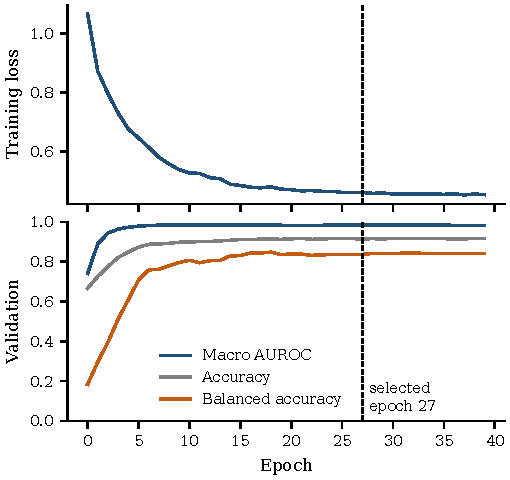
\includegraphics[width=\columnwidth]{figures/training_curves.pdf}
\caption{Training loss (top) and validation metrics (bottom) per epoch, as logged during training, when validation used EMA weights. The dashed line marks epoch 27, the epoch with the highest validation AUROC.}
\label{fig:curves}
\end{figure}

Fig.~\ref{fig:curves} shows the training curves. Validation AUROC reached 0.983 by epoch 7 and then stayed between 0.981 and 0.985 through epoch 39. Its maximum, 0.9847, came at epoch 27. Balanced accuracy kept rising after AUROC flattened, from 0.762 at epoch 7 to between 0.83 and 0.85 from epoch 15 on. The run took 24 minutes and 33 seconds on one NVIDIA GeForce RTX 4070 Ti.

\begin{table}[t]
\caption{Per-class test results, one-vs-rest. Recall is at the argmax, computed from the published per-image predictions.}
\label{tab:perclass}
\centering
\footnotesize
\setlength{\tabcolsep}{3pt}
\begin{tabular}{@{}lrccc@{}}
\toprule
Class & $n$ & AUROC [95\% CI] & AUPRC & Recall \\
\midrule
akiec & 66 & 0.9817 [0.9561, 0.9966] & 0.8834 & 0.697 \\
bcc & 103 & 0.9957 [0.9932, 0.9979] & 0.9022 & 0.913 \\
bkl & 220 & 0.9815 [0.9671, 0.9915] & 0.9316 & 0.891 \\
df & 23 & 0.9981 [0.9954, 0.9999] & 0.9158 & 0.913 \\
mel & 223 & 0.9678 [0.9525, 0.9805] & 0.8584 & 0.825 \\
nv & 1,341 & 0.9809 [0.9732, 0.9869] & 0.9843 & 0.947 \\
vasc & 29 & 1.0000 [0.9999, 1.0000] & 0.9989 & 1.000 \\
\bottomrule
\end{tabular}
\end{table}

\begin{figure}[t]
\centering
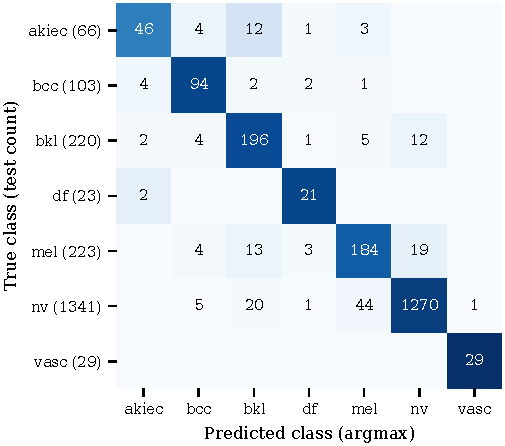
\includegraphics[width=\columnwidth]{figures/confusion_test.pdf}
\caption{Confusion matrix on the 2,005 test images at the argmax. Cell text is the image count, shading the share of the true class.}
\label{fig:confusion}
\end{figure}

Table~\ref{tab:perclass} and Fig.~\ref{fig:confusion} show where the model fails. Melanoma had the lowest AUROC, 0.9678, and 19 of 223 melanomas were called nevi. Of 1,341 nevi, 44 were called melanoma. Actinic keratoses had the lowest recall, 46 of 66, with 12 misses called benign keratoses.

\section{Discussion}

\subsection{Which differences plausibly matter}

Each difference in Table~\ref{tab:setup} is a candidate explanation for the 0.018 gap in AUROC between our run and the best MedMNIST+ value. We ran none of the ablations below, so each paragraph states a hypothesis and the experiment that would test it.

\emph{Pretraining and architecture.} Our backbone was trained with ImageNet-22k labels before ImageNet-1k. Every MedMNIST+ network started from ImageNet-1k or from self-supervised or multimodal weights. MedMNIST+ found that CLIP and DINO pretraining helped linear probes but did not consistently help end-to-end training compared with ImageNet pretraining~\cite{doerrich2025medmnistplus}. The gain may therefore come from the architecture as much as from the pretraining data. Two runs would separate them: our recipe with \texttt{convnext\_small.fb\_in1k}, and our recipe with DenseNet-121 and ImageNet-1k weights.

\emph{Augmentation.} MedMNIST+ trains with no augmentation, which with 7,007 training images invites overfitting, and its early stopping after five epochs without improvement in validation loss may end training before the network adapts. In our view, random resized crops and flips are, with pretraining, one of the two most likely contributors. The test is our recipe with the crop and flips removed.

\emph{Regularization.} Label smoothing, stochastic depth at 0.2, and weight decay of 0.05 all act against overfitting, and their effects overlap with augmentation. One run per component, each removed in turn, would measure them.

\emph{Stopping and selection.} MedMNIST+ keeps the epoch with the lowest validation loss. We train for a fixed 40 epochs and keep the epoch with the highest validation AUROC. Validation loss can rise while ranking still improves, so the two rules can pick different epochs. Fig.~\ref{fig:curves} shows that our validation AUROC was flat within 0.004 from epoch 7 to 39, so we expect selection itself to matter little. Rescoring our run's per-epoch checkpoints under the MedMNIST+ rule would test it, but our pipeline keeps only the selected checkpoint, so this needs a rerun.

\emph{Test-time flips.} We expect averaging the image and its mirror to add little, but we have not measured it. Scoring the released checkpoint with flips turned off would measure it directly, with no retraining.

\emph{EMA.} EMA changed only which epoch was kept. Its effect could be measured by selecting on raw-weight validation AUROC. Given the flat curve, we expect it to be small.

\emph{Seed variation.} MedMNIST+ reports seed standard deviations of 0.0006 to 0.0051 in AUROC for its three best 224-pixel DermaMNIST models. A spread of that size would not close a 0.0126 gap to our lower bound, but our own seed spread is unknown until we train more seeds.

\subsection{Limitations}
\label{sec:limits}

\emph{One run.} We trained once, with seed 0, while the MedMNIST+ values are means of three seeds. Training used \texttt{deterministic: warn} on a GPU, so a rerun is not guaranteed to match bit for bit.

\emph{No ablations.} Every attribution above is untested. The gap could come from one difference or from several together.

\emph{The interval covers test sampling only.} It does not include variation across seeds or training runs.

\emph{Images, not lesions.} The bootstrap treated test images as independent. Correlated images of one lesion would make the true interval wider, and lesions shared between training and test would inflate all scores on this split, ours and the baselines' alike.

\emph{EMA and the reported weights.} The checkpoint holds raw weights, but it was chosen with EMA validation scores. The validation AUROC logged during training at epoch 27 was 0.9847 with EMA weights. Rescoring the saved raw weights gave 0.9840. The rescore also switched AUROC from torchmetrics~\cite{detlefsen2022torchmetrics} in single precision to scikit-learn in double precision, so the 0.0007 gap mixes both changes.

\emph{Imbalance.} Accuracy, 0.918, should be read against the 0.669 of a constant answer. Recall on actinic keratoses (0.697) and melanoma (0.825) is the weakest part of the result.

\emph{Use.} DermaMNIST inherits the CC BY-NC 4.0 license of HAM10000, so the weights are for non-commercial use only. The model is a research artifact, not a medical device, and it has not been validated on clinical data.

\subsection{Reproducibility}

The run was trained with a clean tree at the commit and with the command below, under Windows 11 with Python 3.12.16, PyTorch 2.15.0 (CUDA 13.2), Lightning 2.6.6, timm 1.0.31, and medmnist 3.0.2.
\begin{center}\footnotesize
\texttt{ab39eb9758be4bb65d091fad1d98b521edfbf837}\\[2pt]
\texttt{uv run opendiagnostics fit -c models/dermamnist-convnext/config.yaml}
\end{center}
The checkpoint was rescored, with the selection kept, at commit \texttt{e9f733f}. All reported numbers come from that rescored \texttt{metrics.json}. Code, configuration, and per-image predictions are at \url{https://github.com/isaiah-harville/opendiagnostics} under \path{models/dermamnist-convnext/}. The checkpoint (SHA-256 beginning \texttt{26a4b68b}) is at \url{https://diagnostics.harville.dev/opendiagnostics-weights/dermamnist-convnext/20261126-141911-ab39eb97/checkpoint.ckpt}. The figures are drawn from the committed run files by \path{papers/dermamnist/make_figures.py} with matplotlib~\cite{hunter2007matplotlib}.

\section{Conclusion}

Several changes to the MedMNIST+ training setup, made together, coincided with a DermaMNIST AUROC whose interval lies above every published value we found. Which changes matter is still open. The cheapest test is to score the released checkpoint without flip averaging. The most informative are retraining with the augmentation removed and with an ImageNet-1k backbone, each over three seeds so the results can be set against the MedMNIST+ means.

\section*{Acknowledgment}

Claude, an AI model made by Anthropic, took part in this work. It helped design and run the experiments, wrote parts of the training and evaluation code, analyzed the results, and drafted and revised this paper. Isaiah R. Harville reviewed the work and is responsible for its content.

\bibliographystyle{IEEEtran}
\bibliography{refs}

\end{document}
